\documentclass[journal,12pt,twocolumn]{IEEEtran}
%
\usepackage{setspace}
\usepackage{gensymb}
\usepackage{siunitx}
\usepackage{tkz-euclide} 
\usepackage{textcomp}
\usepackage{standalone}
\usetikzlibrary{calc}
\newcommand\hmmax{0}
\newcommand\bmmax{0}

%\doublespacing
\singlespacing

%\usepackage{graphicx}
%\usepackage{amssymb}
%\usepackage{relsize}
\usepackage[cmex10]{amsmath}
%\usepackage{amsthm}
%\interdisplaylinepenalty=2500
%\savesymbol{iint}
%\usepackage{txfonts}
%\restoresymbol{TXF}{iint}
%\usepackage{wasysym}
\usepackage{amsthm}
%\usepackage{iithtlc}
\usepackage{mathrsfs}
\usepackage{txfonts}
\usepackage{stfloats}
\usepackage{bm}
\usepackage{cite}
\usepackage{cases}
\usepackage{subfig}
%\usepackage{xtab}
\usepackage{longtable}
\usepackage{multirow}
%\usepackage{algorithm}
%\usepackage{algpseudocode}
\usepackage{enumitem}
\usepackage{mathtools}
\usepackage{steinmetz}
\usepackage{tikz}
\usepackage{circuitikz}
\usepackage{verbatim}
\usepackage{tfrupee}
\usepackage[breaklinks=true]{hyperref}
%\usepackage{stmaryrd}
\usepackage{tkz-euclide} % loads  TikZ and tkz-base
%\usetkzobj{all}
\usetikzlibrary{calc,math}
\usepackage{listings}
    \usepackage{color}                                            %%
    \usepackage{array}                                            %%
    \usepackage{longtable}                                        %%
    \usepackage{calc}                                             %%
    \usepackage{multirow}                                         %%
    \usepackage{hhline}                                           %%
    \usepackage{ifthen}                                           %%
  %optionally (for landscape tables embedded in another document): %%
    \usepackage{lscape}     
\usepackage{multicol}
\usepackage{chngcntr}
\usepackage{amsmath}
\usepackage{cleveref}
\usepackage{amsmath}
%\usepackage{enumerate}

%\usepackage{wasysym}
%\newcounter{MYtempeqncnt}
\DeclareMathOperator*{\Res}{Res}
%\renewcommand{\baselinestretch}{2}
\renewcommand\thesection{\arabic{section}}
\renewcommand\thesubsection{\thesection.\arabic{subsection}}
\renewcommand\thesubsubsection{\thesubsection.\arabic{subsubsection}}

\renewcommand\thesectiondis{\arabic{section}}
\renewcommand\thesubsectiondis{\thesectiondis.\arabic{subsection}}
\renewcommand\thesubsubsectiondis{\thesubsectiondis.\arabic{subsubsection}}

% correct bad hyphenation here
\hyphenation{op-tical net-works semi-conduc-tor}
\def\inputGnumericTable{}                                 %%

\lstset{
%language=C,
frame=single, 
breaklines=true,
columns=fullflexible
}
%\lstset{
%language=tex,
%frame=single, 
%breaklines=true
%}
\usepackage{graphicx}
\usepackage{pgfplots}

\begin{document}


\newtheorem{theorem}{Theorem}[section]
\newtheorem{problem}{Problem}
\newtheorem{proposition}{Proposition}[section]
\newtheorem{lemma}{Lemma}[section]
\newtheorem{corollary}[theorem]{Corollary}
\newtheorem{example}{Example}[section]
\newtheorem{definition}[problem]{Definition}
%\newtheorem{thm}{Theorem}[section] 
%\newtheorem{defn}[thm]{Definition}
%\newtheorem{algorithm}{Algorithm}[section]
%\newtheorem{cor}{Corollary}
\newcommand{\BEQA}{\begin{eqnarray}}
\newcommand{\EEQA}{\end{eqnarray}}
\newcommand{\define}{\stackrel{\triangle}{=}}
\bibliographystyle{IEEEtran}
%\bibliographystyle{ieeetr}
\providecommand{\mbf}{\mathbf}
\providecommand{\abs}[1]{\ensuremath{\left\vert#1\right\vert}}
\providecommand{\norm}[1]{\ensuremath{\left\lVert#1\right\rVert}}
\providecommand{\mean}[1]{\ensuremath{E\left[ #1 \right]}}
\providecommand{\pr}[1]{\ensuremath{\Pr\left(#1\right)}}
\providecommand{\qfunc}[1]{\ensuremath{Q\left(#1\right)}}
\providecommand{\sbrak}[1]{\ensuremath{{}\left[#1\right]}}
\providecommand{\lsbrak}[1]{\ensuremath{{}\left[#1\right.}}
\providecommand{\rsbrak}[1]{\ensuremath{{}\left.#1\right]}}
\providecommand{\brak}[1]{\ensuremath{\left(#1\right)}}
\providecommand{\lbrak}[1]{\ensuremath{\left(#1\right.}}
\providecommand{\rbrak}[1]{\ensuremath{\left.#1\right)}}
\providecommand{\cbrak}[1]{\ensuremath{\left\{#1\right\}}}
\providecommand{\lcbrak}[1]{\ensuremath{\left\{#1\right.}}
\providecommand{\rcbrak}[1]{\ensuremath{\left.#1\right\}}}
\theoremstyle{remark}
\newtheorem{rem}{Remark}
\newcommand{\sgn}{\mathop{\mathrm{sgn}}}
\providecommand{\res}[1]{\Res\displaylimits_{#1}} 
%\providecommand{\norm}[1]{\lVert#1\rVert}
\providecommand{\mtx}[1]{\mathbf{#1}}
\providecommand{\fourier}{\overset{\mathcal{F}}{ \rightleftharpoons}}
%\providecommand{\hilbert}{\overset{\mathcal{H}}{ \rightleftharpoons}}
\providecommand{\system}{\overset{\mathcal{H}}{ \longleftrightarrow}}
	%\newcommand{\solution}[2]{\textbf{Solution:}{#1}}
\newcommand{\solution}{\noindent \textbf{Solution: }}
\newcommand{\cosec}{\,\text{cosec}\,}
\providecommand{\dec}[2]{\ensuremath{\overset{#1}{\underset{#2}{\gtrless}}}}
\newcommand{\myvec}[1]{\ensuremath{\begin{pmatrix}#1\end{pmatrix}}}
\newcommand{\mydet}[1]{\ensuremath{\begin{vmatrix}#1\end{vmatrix}}}
%\numberwithin{equation}{section}
\numberwithin{equation}{subsection}
%\numberwithin{problem}{section}
%\numberwithin{definition}{section}
\makeatletter
\@addtoreset{figure}{problem}
\makeatother
\let\StandardTheFigure\thefigure
\let\vec\mathbf
%\renewcommand{\thefigure}{\theproblem.\arabic{figure}}
\renewcommand{\thefigure}{\theproblem}
%\setlist[enumerate,1]{before=\renewcommand\theequation{\theenumi.\arabic{equation}}
%\counterwithin{equation}{enumi}
%\renewcommand{\theequation}{\arabic{subsection}.\arabic{equation}}
\def\putbox#1#2#3{\makebox[0in][l]{\makebox[#1][l]{}\raisebox{\baselineskip}[0in][0in]{\raisebox{#2}[0in][0in]{#3}}}}
     \def\rightbox#1{\makebox[0in][r]{#1}}
     \def\centbox#1{\makebox[0in]{#1}}
     \def\topbox#1{\raisebox{-\baselineskip}[0in][0in]{#1}}
\vspace{3cm}
\title{Hyperbola}
\maketitle
\newpage
%\tableofcontents
\bigskip
\renewcommand{\thefigure}{\theenumi}
\renewcommand{\thetable}{\theenumi}
\begin{abstract}
This document contains solution of Problem Loney\brak{314,7}
\end{abstract}
Download latex-tikz codes from 
%
\begin{lstlisting}
https://github.com/ayushkesh/Matrix-Theory-EE5609/tree/master/A7
\end{lstlisting}
\section{\textbf{Question}}
Find the asymptotes of the hyperbola given below and also the equations to their conjugate hyperbolas.\\
$8x^2+10xy-3y^2-2x+4y-2=0$
\section{Solution}
The above equation can be expressed in the form 
\begin{align}
\vec{x}^T\vec{V}\vec{x}+2\vec{u}^T\vec{x}+f&=0\label{2.2} \label{eq1}
\intertext{Comparing equation we get}
    \vec{V}=\vec{V}^T&=\myvec{8 & 5 \\ 5 &-3}\label{eqv}\\
    \vec{u}&=\myvec{-1 \\2 }\label{equ}\\
    f&=-2\label{eqfv}
\end{align}   
Expanding the Determinant of \vec{V}.
\begin{align}
    \Delta_{V} &= \begin{array}{|cc|}
8 &5\\5 & -3
\end{array}<0\label{eq:hyp}
\end{align}
Hence from \eqref{eq:hyp} given
equation represents the hyperbola
The characteristic equation of $\vec{V}$ is obtained by evaluating the determinant 
\begin{align}
       \begin{array}{|c|}
V-\lambda\vec{I}
\end{array}&=0\\
   \begin{array}{|cc|}
8-\lambda & 5 \\ 5 & -3-\lambda
\end{array}&=0\\
    \brak{8-\lambda}\brak{-3-\lambda}-25=0\\
    \lambda_{1}= \frac{5+\sqrt{221}}{2}\label{eq:matrix_l1}\\
    \lambda_{2}= \frac{5-\sqrt{221}}{2}\label{eq:matrix_l2}
\end{align}
The eigenvector $\vec{p}$ is defined as 
\begin{align}
    \vec{V}\vec{p}&=\lambda\vec{p}\\
    \implies (\vec{V}-\lambda\vec{I})\vec{p}&=0\label{eq:7/eqev}
\end{align}
For $\lambda_1=\frac{5+\sqrt{221}}{2}$ ,
\begin{align}
    (\vec{V}-\lambda_1\vec{I})=\myvec{\frac{11-\sqrt{221}}{2} & 5 \\5 & \frac{-11-\sqrt{221}}{2}}
\end{align}
By row reduction , 
\begin{align}
    &\myvec{\frac{11-\sqrt{221}}{2} & 5 \\5 & \frac{-11-\sqrt{221}}{2}}\\
    %&\xleftrightarrow{\frac{R_1}{\frac{\sqrt{533}+2}{2}}}\\
    &\xleftrightarrow{R_1\leftarrow R_2}
    \myvec{\frac{-11-\sqrt{221}}{2} & 5 \\ \frac{11-\sqrt{221}}{2} & 5}\\
 &\xleftrightarrow{R_2\leftarrow R_2-\frac{11-\sqrt{221}}{10}R_{1}}
    \myvec{5 & \frac{-11-\sqrt{221}}{2} \\ 0& 0}\\
     &\xleftrightarrow{R_1\leftarrow R_1/5}
    \myvec{1 & \frac{-11-\sqrt{221}}{10} \\ 0& 0}
    \label{eq:7/eqs1}
\end{align}
Subsituting equation \ref{eq:7/eqs1} in equation \ref{eq:7/eqev} we get
\begin{align}
        & \myvec{1 & \frac{-11-\sqrt{221}}{10} \\ 0& 0}\myvec{v_1 \\ v_2}=\myvec{0 \\ 0}\label{eq:7/eqei1}
\end{align}
Where, $\vec{p}=\myvec{v_1\\v_2}$
Let $v_2=t$
\begin{align}
    v_1&=\frac{t(11+\sqrt{221})}{10}
\end{align}
Eigen vector $\vec{p_1}$ is given by
\begin{align}
    \vec{p_1}&=\myvec{\frac{t(11+\sqrt{221})}{10} \\ t}
\end{align}
Let $t=1$, we get
\begin{align}
        \vec{p_1}&=\myvec{\frac{11+\sqrt{221}}{10} \\1 }\label{eq:es71/eqp1}
\end{align}
For $\lambda_2=\frac{5-\sqrt{221}}{2}$ ,
\begin{align}
    (\vec{V}-\lambda_2\vec{I})=\myvec{\frac{11+\sqrt{221}}{2} & 5 \\5 & \frac{-11+\sqrt{221}}{2}}
\end{align}
By row reduction , 
\begin{align}
     \myvec{\frac{11+\sqrt{221}}{2} & 5 \\5 & \frac{-11+\sqrt{221}}{2}}
    \xleftrightarrow{R_1\leftarrow R_2+ \frac{11-\sqrt{221}}{10}R_1}
     \myvec{\frac{11+\sqrt{221}}{2} &5\\ 0& 0}\\  
 \xleftrightarrow{R_1\leftarrow
 \frac{R_1}{\frac{11+\sqrt{221}}{10}}}
    \myvec{1 & \frac{10}{11+\sqrt{221}} \\ 0& 0}
    \label{eq:es71/eqs2}
\end{align} 
Substiuting equation \ref{eq:es71/eqs2} in equation \ref{eq:7/eqev} we get 
\begin{align}
    &\myvec{1 & \frac{10}{11+\sqrt{221}} \\0 & 0}\myvec{v_1 \\ v_2}=\myvec{0 \\ 0}
%\label{eq:es71/eqei1}
\end{align}
Where, $\vec{p}=\myvec{v_1\\v_2}$
Let $v_2=t$
\begin{align}
    v_1&=\frac{-t\brak{10}}{11+\sqrt{221}}
\end{align}
Eigen vector $\vec{p_2}$ is given by
\begin{align}
        \vec{p_2}&=\myvec{\frac{-t\brak{10}}{11+\sqrt{221}} \\ t}
\end{align}
Let $t=1$, we get 
\begin{align}
    \vec{p_2}&=\myvec{\frac{\brak{-10}}{11+\sqrt{221}} \\1 }\label{eq:es71/eqp2}
\end{align}
By eigen decompostion $\vec{V}$ can be represented by
\begin{align}
    \vec{V}&=\vec{P}\vec{D}\vec{P}^T\label{eq:es71/eqsubs}
\end{align}
where 
\begin{align}
        \vec{P}&=\myvec{\vec{p_1} & \vec{p_2}}\label{eq:es71/eqp}\\
    \vec{D}&=\myvec{\lambda_1 & 0 \\0 & \lambda_2}\label{eq:es71/eqD}
\end{align}
Substituting equations \ref{eq:es71/eqp1}, \ref{eq:es71/eqp2} in equation \ref{eq:es71/eqp} we get 
\begin{align}
    \vec{P}&=\myvec{\frac{11+\sqrt{221}}{10} & \frac{-10}{11+\sqrt{221}} \\1 & 1}\label{eq:es71/eqP}
\end{align}
Substituting equations \ref{eq:matrix_l1}, \ref{eq:matrix_l2} in \ref{eq:es71/eqD} we get
\begin{align}
       \vec{D}&=\myvec{\frac{5+\sqrt{221}}{2} & 0\\0 & \frac{5-\sqrt{221}}{2}}\label{eq:es71/eqDD}
\end{align}
Centre of the hyperbola is given by 
\begin{align}
    \vec{c}&=-\vec{V}^{-1}\vec{u}\\
    \implies\vec{c}&=-\myvec{\frac{3}{49}&\frac{5}{49}\\\frac{5}{49}&\frac{-8}{49}}\myvec{-1 \\ 2}\\
    \implies\vec{c}&=\myvec{\frac{-3}{49}&\frac{-5}{49}\\\frac{-5}{49}&\frac{8}{49}}\myvec{-1 \\ 2}\\
    \implies\vec{c}&=\myvec{\frac{-1}{7}\\\frac{3}{7}}
\end{align}
Since,
\begin{align}
    \vec{u}^T\vec{V}^{-1}\vec{u}-f = 1 > 0\label{eq:es71/cond}
\end{align} 
there isn't a need to swap axes
In hyperbola,
\begin{align}
axes=
\begin{cases}
\sqrt{\frac{\vec{u}^T\vec{V}^{-1}\vec{u}-f}{\lambda_1}}\\ \sqrt{\frac{f-\vec{u}^T\vec{V}^{-1}\vec{u}}{\lambda_2}}
\end{cases}
\end{align}
From above equations we can say that,
\begin{align}
\sqrt{\frac{\vec{u}^T\vec{V}^{-1}\vec{u}-f}{\lambda_1}}=\sqrt{ \frac{2}{5+\sqrt{221}}}\\
\sqrt{\frac{f-\vec{u}^T\vec{V}^{-1}\vec{u}}{\lambda_2}}=\sqrt{ \frac{2}{5-\sqrt{221}}}
\end{align}
Now we have,
\begin{align}
    \vec{y}^T\vec{D}\vec{y}&=\vec{u}^T\vec{V}^{-1}\vec{u}-f\label{eq:es71/fi}
\end{align}
where ,
\begin{align}
    \vec{y}&=\vec{P}^T(\vec{x}-\vec{c})
\end{align}
To get $\vec{y}$,
\begin{align}
\vec{y}&=\vec{P}^T\vec{x}-\vec{P}^T\vec{c}\\
    \vec{y}&= \myvec{\frac{11+\sqrt{221}}{10} & 1 \\ \frac{-10}{11+\sqrt{221}} & 1}\vec{x}-\myvec{\frac{11+\sqrt{221}}{10} & 1 \\ \frac{-10}{11+\sqrt{221}} & 1}\myvec{\frac{-1}{7}\\\frac{3}{7}}\\
    \vec{y}&=\myvec{\frac{11+\sqrt{221}}{10} & 1 \\ \frac{-10}{11+\sqrt{221}} & 1}\vec{x}-\myvec{\frac{-11-\sqrt{221}}{70}+\frac{3}{7} \\ \frac{10}{(7)11+(7)\sqrt{221}}+\frac{3}{7}}
\end{align}
Subsituting the eqauations \eqref{eq:es71/cond}, \eqref{eq:es71/eqDD} in equation \eqref{eq:es71/fi}
\begin{align}
   \implies\vec{y}^T\myvec{\frac{5+\sqrt{221}}{2} & 0 \\0 & \frac{5-\sqrt{221}}{2}}\vec{y}+2&=0
\end{align}
\subsection{Asymptotes of hyperbola}
Equation of a hyperbola and the combined equation of the Asymptotes differ only in the constant term.
\begin{align}
 8x^2+10xy-3y^2−2x+4y+K=0   
\end{align}
The above equation can be expressed in the form 
\begin{align}
\vec{x}^T\vec{V}\vec{x}+2\vec{u}^T\vec{x}+f&=0\label{2.2} \label{eq1}
\intertext{Comparing equation we get}
    \vec{V}=\vec{V}^T&=\myvec{8 & 5 \\ 5 &-3}\label{eq:es1/eqv}\\
    \vec{u}&=\myvec{-1 \\2 }\label{eq:equ}\\
    f&=K\label{eq:es1/eqfv}
\end{align}   
\begin{align}
\Delta&=\begin{array}{|ccc|}
8 & 5 & -1\\ 5& -3 & 2\\ -1 & 2 & K
\end{array}\\
\implies K&=-1
\end{align}
Similar way expanding the Determinant of \vec{V}.
\begin{align}
    \Delta_{V} &= \begin{array}{|cc|}
8 &5\\5 & -3
\end{array}<0\label{eq:es/17/hyp}
\end{align}
From \eqref{eq:es/17/hyp} we could say that the given equation represents two straight lines
Let the equations of lines be,
\begin{align}
	\brak{\vec{n_1}^T \vec{x} - c_1}\brak{\vec{n_1}^T \vec{x} - c_1} =
        \vec{x}^{T}\vec{Vx} + 2\vec{u}^{T}\vec{x} + f=0\label{eq:eql7/03}
\end{align}
\begin{align}
\brak{\vec{n_1}^T\vec{x}-c_1}\brak{\vec{n_2}^T\vec{x}-c_2}
&=\vec{x}^T\myvec{8 & 5 \\ 5 & -3}\vec{x}\notag\\
+2\myvec{-1 & 2}\vec{x}-1\label{equate}\\
    \vec{n_1}*\vec{n_2} = \myvec{a\\2b\\c} &= \myvec{8\\10\\-3}\label{conv}\\
    c_2\vec{n_1}+c_1\vec{n_2}&=-2\myvec{-1\\2}\label{eq17/c1c2}\\
    c_1c_2&=-1
\end{align}
The slopes of the lines are given by the roots of the polynomial 
\begin{align}
    &cm^2+2bm+a=0\label{e}\\
    \implies m_i&=\frac{-b\pm{\sqrt{-\Delta_{V}}}}{c}\\
    \vec{n_i}&=k\myvec{-m_i\\1}
\end{align}
Substituting the given data in above equations \eqref{e} we get,
\begin{align}
    &-3m^2+10m+8=0\\
    m_1&=4,  m_2=\frac{-2}{3}\\
   &= \vec{n_1}=\myvec{-4\\ 1}, \vec{n_2}=\myvec{-2\\-3} \label{eq:normal1}
\intertext{We know that,}
& \vec{n_1}\ast \vec{n_2} = \myvec{a\\2b\\c} \label{eq:conv1}
\end{align}
Verification using Toeplitz matrix, From equation \eqref{eq:normal1}
\begin{align}
    \vec{n_1}=\myvec{-4&0\\1&-4\\0&-1}
    \vec{n_2}=\myvec{-2\\-3}\label{eq:conv2}\\
\implies \myvec{-4&0\\1&-4\\0&1}\myvec{0\\ -1} = \myvec{8\\10\\-3} = \myvec{a\\2b\\c}\label{eq:conv3}
\end{align}
$\implies$ Equation \eqref{eq:normal1} satisfies \eqref{eq:conv1}\\
$c_1$ and $c_2$ can be obtained as,
\begin{align}
\myvec{\vec{n_1} & \vec{n_2}}\myvec{c_2\\c_1}&=-2\vec{u} \label{eq:aug1}
\end{align}
Substituting \eqref{eq:normal1} in \eqref{eq:aug1}, the augmented matrix is,
\begin{align}
\myvec{-4 & -2 & -2 \\ 1 & -3 & 4}
\xleftrightarrow[R_2\leftarrow R_2-R_1]{R_1\leftarrow -R_1/4}
\myvec{1 &\frac{1}{2} &\frac{1}{2} \\ 0 & -\frac{7}{2} & \frac{7}{2}} \label{eq:aug5}\\
\xleftrightarrow[R_1\leftarrow R_1-\frac{1}{2}R_2]{R_2\leftarrow -\frac{2}{7}R_2}
\myvec{1 &0 &1 \\ 0& 1 & -1} \label{eq:aug2}\\
\implies c_1 = 1, c_2=-1 \label{eq:const1}
\end{align}
Equations \eqref{eq:eql7/03}, can be modified as,from \eqref{eq:normal1} and \eqref{eq:const1} in we get,
\begin{align}
    \myvec{-4 & 1}\vec{x}&=1\\
    \myvec{-2 & -3}\vec{x}&=-1
\end{align}
\begin{multline}
\implies \brak{-4x+y-1}\brak{-2x-3y+1}= 0\\
\implies \boxed{\brak{4x-y+1}\brak{2x+3y-1} = 0} \label{eq:line1}
\end{multline}
The angle between the lines can be expressed as, 
\begin{align}
	\vec{n_1}=\myvec{-4\\1} , \quad \vec{n_2}=\myvec{-2\\-3}\\
	\cos\theta=\frac{\vec{n_1}^T\vec{n_2}}{\norm{\vec{n_1}}\norm{\vec{n_2}}} \\
	\implies \quad \theta=\cos^{-1}({\frac{0}{\sqrt{221}}}) = 90\degree.
\end{align}
\subsection{Equation of Asymptotes}
The characteristic equation of $\vec{V}$ is obtained by evaluating the determinant \eqref{eq:es1/eqv}
\begin{align}
       \begin{array}{|c|}
V-\lambda\vec{I}
\end{array}&=0\\
   \begin{array}{|cc|}
8-\lambda & 5 \\ 5 & -3-\lambda
\end{array}&=0\\
    \brak{8-\lambda}\brak{-3-\lambda}-25=0\\
    \lambda_{1}= \frac{5+\sqrt{221}}{2}\\
    \lambda_{2}= \frac{5-\sqrt{221}}{2}
\end{align}
The eigenvector $\vec{p}$ is defined as 
\begin{align}
    \vec{V}\vec{p}&=\lambda\vec{p}\\
    \implies (\vec{V}-\lambda\vec{I})\vec{p}&=0\label{eq:es/2701}
\end{align}
For $\lambda_1=\frac{5+\sqrt{221}}{2}$ ,
\begin{align}
    (\vec{V}-\lambda_1\vec{I})=\myvec{\frac{11-\sqrt{221}}{2} & 5 \\5 & \frac{-11-\sqrt{221}}{2}}
\end{align}
By row reduction , 
\begin{align}
    &\myvec{\frac{11-\sqrt{221}}{2} & 5 \\5 & \frac{-11-\sqrt{221}}{2}}\\
    %&\xleftrightarrow{\frac{R_1}{\frac{\sqrt{533}+2}{2}}}\\
    &\xleftrightarrow{R_1\leftarrow R_2}
    \myvec{\frac{-11-\sqrt{221}}{2} & 5 \\ \frac{11-\sqrt{221}}{2} & 5}\\
 &\xleftrightarrow{R_2\leftarrow R_2-\frac{11-\sqrt{221}}{10}R_{1}}
    \myvec{5 & \frac{-11-\sqrt{221}}{2} \\ 0& 0}\\
     &\xleftrightarrow{R_1\leftarrow R_1/5}
    \myvec{1 & \frac{-11-\sqrt{221}}{10} \\ 0& 0}
    \label{eq:es27/02}
\end{align}
Subsituting equation \ref{eq:es27/02} in equation \ref{eq:es/2701} we get
\begin{align}
        & \myvec{1 & \frac{-11-\sqrt{221}}{10} \\ 0& 0}\myvec{v_1 \\ v_2}=\myvec{0 \\ 0}\label{eq:es27/eqei1}
\end{align}
Where, $\vec{p}=\myvec{v_1\\v_2}$
Let $v_2=t$
\begin{align}
    v_1&=\frac{t(11+\sqrt{221})}{10}
\end{align}
Eigen vector $\vec{p_1}$ is given by
\begin{align}
    \vec{p_1}&=\myvec{\frac{t(11+\sqrt{221})}{10} \\ t}
\end{align}
Let $t=1$, we get
\begin{align}
        \vec{p_1}&=\myvec{\frac{11+\sqrt{221}}{10} \\1 }\label{eq:es27/eqp1}
\end{align}
For $\lambda_2=\frac{5-\sqrt{221}}{2}$ ,
\begin{align}
    (\vec{V}-\lambda_2\vec{I})=\myvec{\frac{11+\sqrt{221}}{2} & 5 \\5 & \frac{-11+\sqrt{221}}{2}}
\end{align}
By row reduction , 
\begin{align}
    \myvec{\frac{11+\sqrt{221}}{2} & 5 \\5 & \frac{-11+\sqrt{221}}{2}}
    \xleftrightarrow{R_1\leftarrow R_2+ \frac{11-\sqrt{221}}{10}R_1}
     \myvec{\frac{11+\sqrt{221}}{2} &5\\ 0& 0}\\  
 \xleftrightarrow{R_1\leftarrow
 \frac{R_1}{\frac{11+\sqrt{221}}{10}}}
    \myvec{1 & \frac{10}{11+\sqrt{221}} \\ 0& 0}
    \label{eq:es27eqs02}
\end{align}
Subsituting equation \ref{eq:es27eqs02} in equation \ref{eq:es/2701} we get 
\begin{align}
    &\myvec{1 & \frac{10}{11+\sqrt{221}} \\0 & 0}\myvec{v_1 \\ v_2}=\myvec{0 \\ 0}
%\label{eq:es27/eqei1}
\end{align}
Where, $\vec{p}=\myvec{v_1\\v_2}$
Let $v_2=t$
\begin{align}
    v_1&=\frac{-t\brak{10}}{11+\sqrt{221}}
\end{align}
Eigen vector $\vec{p_2}$ is given by
\begin{align}
        \vec{p_2}&=\myvec{\frac{-t\brak{10}}{11+\sqrt{221}} \\ t}
\end{align}
Let $t=1$, we get 
\begin{align}
    \vec{p_2}&=\myvec{\frac{\brak{-10}}{11+\sqrt{221}} \\1 }\label{eq:es27/eqp2}
\end{align}
By eigen decompostion $\vec{V}$ can be represented by
\begin{align}
    \vec{V}&=\vec{P}\vec{D}\vec{P}^T\label{eq:es27/eqsubs}
\end{align}
where 
\begin{align}
        \vec{P}&=\myvec{\vec{p_1} & \vec{p_2}}\label{eq:es27/eqp}\\
    \vec{D}&=\myvec{\lambda_1 & 0 \\0 & \lambda_2}\label{eq:es27/eqD}
\end{align}
Substituting equations \ref{eq:es27/eqp1}, \ref{eq:es27/eqp2} in equation \ref{eq:es27/eqp} we get 
\begin{align}
    \vec{P}&=\myvec{\frac{11+\sqrt{221}}{10} & \frac{-10}{11+\sqrt{221}} \\1 & 1}\label{eq:es27/eqP}
\end{align}
\begin{align}
       \vec{D}&=\myvec{\frac{5+\sqrt{221}}{2} & 0\\0 & \frac{5-\sqrt{221}}{2}}\label{eq:es27/eqDD}
\end{align}
Centre of the hyperbola is given by 
\begin{align}
    \vec{c}&=-\vec{V}^{-1}\vec{u}\\
    \implies\vec{c}&=-\myvec{\frac{3}{49}&\frac{5}{49}\\\frac{5}{49}&\frac{-8}{49}}\myvec{-1 \\ 2}\\
    \implies\vec{c}&=\myvec{\frac{-3}{49}&\frac{-5}{49}\\\frac{-5}{49}&\frac{8}{49}}\myvec{-1 \\ 2}\\
    \implies\vec{c}&=\myvec{\frac{-1}{7}\\\frac{3}{7}}
\end{align}
Since,
\begin{align}
    \vec{u}^T\vec{V}^{-1}\vec{u}-f = 0\label{eq:es27/cond}
\end{align} 
Now,
\begin{align}
    \vec{y}^T\vec{D}\vec{y}&=\vec{u}^T\vec{V}^{-1}\vec{u}-f\label{eq:es27/fi}
\end{align}
where ,
\begin{align}
    \vec{y}&=\vec{P}^T(\vec{x}-\vec{c})
\end{align}
To get $\vec{y}$,
\begin{align}
\vec{y}&=\vec{P}^T\vec{x}-\vec{P}^T\vec{c}\\
    \vec{y}&= \myvec{\frac{11+\sqrt{221}}{10} & 1 \\ \frac{-10}{11+\sqrt{221}} & 1}\vec{x}-\myvec{\frac{11+\sqrt{221}}{10} & 1 \\ \frac{-10}{11+\sqrt{221}} & 1}\myvec{\frac{-1}{7}\\\frac{3}{7}}\\
    \vec{y}&=\myvec{\frac{11+\sqrt{221}}{10} & 1 \\ \frac{-10}{11+\sqrt{221}} & 1}\vec{x}-\myvec{\frac{-11-\sqrt{221}}{70}+\frac{3}{7} \\ \frac{10}{(7)11+(7)\sqrt{221}}+\frac{3}{7}}
\end{align}
Subsituting the eqauations \eqref{eq:es27/cond}, \eqref{eq:es27/eqDD} in equation \eqref{eq:es27/fi}
Equation of asymptotes is
\begin{align}
    \implies \vec{y}^T\myvec{\frac{5+\sqrt{221}}{2} & 0 \\0 & \frac{5-\sqrt{221}}{2}}\vec{y}+1&=0
\end{align}
And the Equations of Conjugate hyperbola is 2(Equation of Asymptotes)- Equation of hyperbola. 
\begin{align}
    \implies \vec{y}^T\myvec{\frac{5+\sqrt{221}}{2} & 0 \\0 & \frac{5-\sqrt{221}}{2}}\vec{y}&=0
\end{align}
\renewcommand{\thefigure}{1}
\begin{figure}[h]
    \centering
    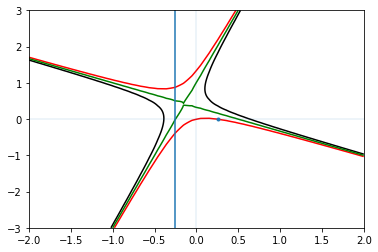
\includegraphics[width=\columnwidth]{A7_4.png}
    \caption{Hyperbola with assymptotes and its conjugate}
    \label{Fig :1}
\end{figure}
Python Code 
\begin{lstlisting}
https://github.com/ayushkesh/Matrix-Theory-EE5609/blob/master/A7/codes/A7_4.ipynb
\end{lstlisting}
\end{document}
